
\subsubsection{Pakovanje porudžbina}
	\begin{figure}[H]
		\begin{center}
			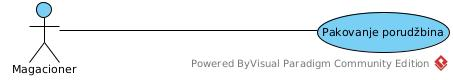
\includegraphics[width=\textwidth]{uc_packaging}
			\caption{Dijagram slučaja upotrebe pakovanja porudžbina}		
		\end{center}
	\end{figure}
	\begin{itemize}
		\item{Kratak opis:} 
		\begin{itemize}
			\item{Magacioner pakuje porudžbine u pakete za isporuku.}
		\end{itemize}
		
		\item{Učesnici:} 
		\begin{itemize}
			\item{Magacioner}
		\end{itemize}		

		\item{Preduslovi:}
		\begin{itemize}
			\item{Magacioner je prijavljen na sistem i ima neupakovanih porudžbina. U magacinu ima dovoljno potrebnih namirnica da se upakuju sve porudžbine.}
		\end{itemize}
		
		\item{Postuslovi:}
		\begin{itemize}
			\item{Nema neupakovanih porudžbina.}
		\end{itemize}
		
		\item{Osnovni tok:}
		\begin{enumerate}
			\item{Magacioner proverava listu neupakovanih porudžbina.}
			\item{Magacioner preuzima jednu porudžbinu i beleži to u sistemu.}
			\item{Sistem štampa identifikacioni broj porudžbine.}
			\item{Magacioner pakuje paket i obeležava ga identifikacionim brojem.}
			\item{Magacioner beleži da je završio pakovanje porudžbine i da je paket spreman za dostavu.}
			\item{Sistem ažurira stanje zaliha u magacinu na osnovu spiska porudžbine.}
			\item{Sistem ažurira status porudžbine.}


			\textit{Koraci 1-6 se ponavljaju sve dok ima nedostavljenih paketa.}
		\end{enumerate}
		\item{Dodatne informacije:}
		\begin{itemize}
			\item{Identifikacioni broj porudžbine se automatski generiše pri konstrukciji porudžbine u sistemu.}
		\end{itemize}
	\begin{figure}[H]
		\begin{center}
			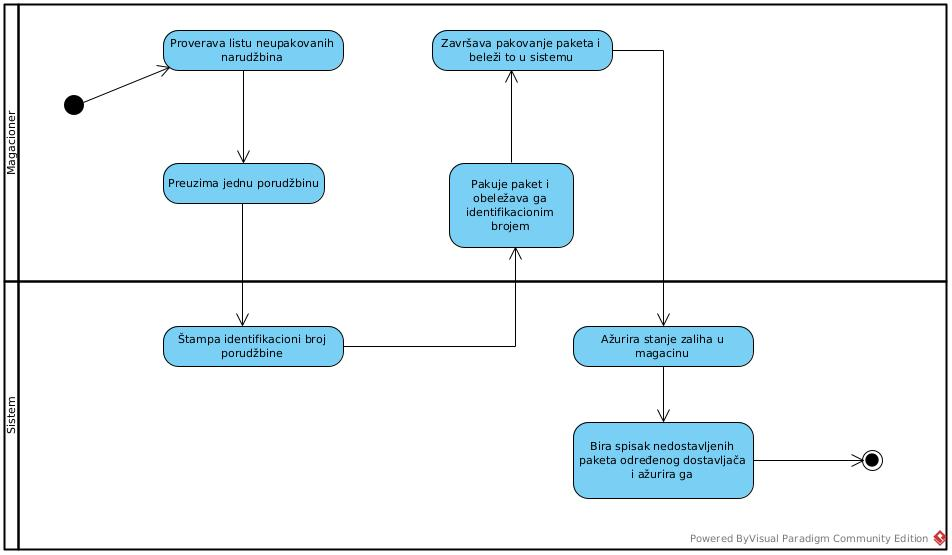
\includegraphics[width=\textwidth]{activity_packaging}
			\caption{Dijagram aktivnosti pakovanja porudžbina}		
		\end{center}
	\end{figure}
	\end{itemize}
